\documentclass[11pt]{article}
\usepackage[margin=1in]{geometry}
\usepackage{enumerate}
\usepackage{framed}
\usepackage{multirow}
\usepackage{multicol}
\usepackage{bm}
\usepackage{amssymb}
\usepackage{amsmath}
\usepackage{amsthm}
\usepackage{multicol}
\usepackage{graphicx}
\setlength{\columnsep}{1in}
\begin{document}

\newcommand{\Name}[1]{\noindent \textbf{Name:} #1 \\}
\newcommand{\pderiv}[2]{\frac{\partial #1}{\partial #2}}
\newcommand{\psderiv}[3]{\frac{\partial^2 #1}{\partial #2 \partial #3}}

\begin{center}
	\bf
	Machine Learning \\
	Computer Science 158 \\
	Spring 2017 \\
	\rm
	Project 6\\
	Due: March 8 at 11:59 PM \\
\end{center}
\noindent \textbf{Name: Varsha Kishore and Savannah Baron} \\
\begin{enumerate}
\item Feature Extraction \\
Code complete!
\item Hyperparameter Selection for Linear SVM
\begin{enumerate}
\item Code complete!
\item As we discussed in class, when training using accuracy as the measure, 
the most accurate approach can be to classify everything as the majority. So, if we 
keep the proportion the same no one fold will have an advantage over the other while
training in terms of ratio of majority to minority. 
\item Code complete!
\item Table 1- best setting for $C$ using Linear SVM:\\
\begin{tabular}{| l | c | c | c | c | c | c |}
  \hline		
  C & accuracy & F1-score & AUROC & precision & sensitivity & specificity \\
  \hline
  $10^{-3}$ & 0.6554 & 0.7918 & 0.8649 & 0.6554 & 1.0 & 0.0 \\
  $10^{-2}$ & 0.7749 & 0.8454 & 0.8654 & 0.7672 & 0.9427 & 0.4559  \\
  $10^{-1}$ &  0.8248 & 0.8715 & 0.8981 & 0.8393 & 0.9073 & 0.668 \\
  $10^{0}$ &  0.8445 & 0.8832 & 0.9101 & 0.8692 & 0.8991 & 0.7408 \\
  $10^{1}$ &  0.8391 & 0.8796 & 0.9086 & 0.8623 & 0.8991 & 0.7252 \\
  $10^{2}$ &  0.8391 & 0.8796 & 0.9086 & 0.8623 & 0.8991 & 0.7252 \\
  \hline
  Best C & 1 & 1 & 1 & 1 & 0.001 & 1 \\
  \hline  
\end{tabular}

\end{enumerate}
\item Hyperparameter Selection for RBF Kernel SVM
\begin{enumerate}[(a)]
\item $\gamma = \frac{1}{2\sigma^2}$. When $\sigma^2$ increases, regularization increases. So, as $\gamma$
increases, regularization decreases. This means that if we are in high bias, increasing $\gamma$ will 
increase generalization. If we are in high variance, decreasing $\gamma$ will increase generalization. 
\item We chose $C$ to range from 0.001 to $10^6$. We used high $C$ values for low regularization, and 
low values for high regularization, in order to cover all possibilities that our model might need. We chose
the same range for gamma for the same reasons. 
\item Table 2- best setting for $C$ and $\gamma$ using RBF SVM: \\

\begin{tabular}{| l | c | c | c |}
\hline
Metric & Score & $\gamma$ & $c$ \\
\hline
Accuracy & 0.8481 & 0.01 & 100.0 \\
F1-score & 0.8867 & 0.01 & 100.0 \\
Auroc & 0.9140 & 0.01 & 100.0 \\
Precision & 0.8684 & 0.01 & 100.0 \\
Sensitivy & 1.0000 & 0.001 & 0.001 \\
Specificity & 0.7359 & 0.01 & 100.0 \\
\hline
\end{tabular}
\end{enumerate}
\item Test Set Performance
\begin{enumerate}[(a)]
\item Using table $1$, we choose $C=1$ for the linear SVM because we can see from the table that the scores for the different metrics are highest when $C=1$ for all metrics except sensitivity. Using table $2$, we choose $C=100$ and $\gamma = 0.01$ for the RBF SVM because we can see from the table that  the best $C$ and best $\gamma$ is $100$ and $0.01$ respectively for all metrics except sensitivity. 
\item Code complete!
\item Test set performance of classifiers: \\
\begin{tabular}{| c | c | c | c | c |}
\hline
Metric & Type &Score & Lower & Upper \\
\hline
Accuracy & Linear & $0.7571$ & $0.6571$ & $0.8432$ \\
Accuracy & RBF & $0.7571$ & $0.6571$ & $0.8432$ \\
F1-score & Linear & $0.8247$ & $0.7368$ & $0.9020$ \\
F1-score & RBF & $0.8283$ & $0.7391$ & $0.9027$ \\
auroc & Linear & $0.8101$ & $0.6910$ & $0.9157$ \\
auroc & RBF & $0.8204$ & $0.6959$ & $0.9212$ \\
precision & Linear & $0.8696$ & $0.7674$ & $0.9574$ \\
precision & RBF & $0.8542$ & $0.7556$ & $0.9535$ \\
sensitivity & Linear & $0.7843$ & $0.6667$ & $0.8800$ \\
sensitivity & RBF & $0.8039$ & $0.6923$ & $0.9074$ \\
specificity & Linear & $0.6842$ & $0.4614$ & $0.8889$ \\
specificity & RBF & $0.6316$ & $0.3747$ & $0.8462$ \\
\hline
\end{tabular} \\
\end{enumerate}
\item Explanation \\
We have a set of tweets that consist of both positive and negative movie review tweets. We are looking at word choices used in positive and negative tweets. Based on this, we can then automatically predict whether any other tweet is positive or negative depending on what words are in it. \\
Imagine we have two twitter users- one who likes all the movies and uses a lot of emoji's and another who hates all the movies and does not use emoji's. Then, we could incorrectly say that having a lot of emoji's is a positive movie review tweet. This is incorrect. In order to prevent this we should not give too much importance to the emoji's. So, we ran experiments to find out how much importance we need to give to different word choices. 
\item Contest\\
First, we wanted to see whether we were in high bias or high variance, in order to know what sorts of improvements would be best to pursue. We created a learning curve of how much data was used in the training set versus the train and test errors.

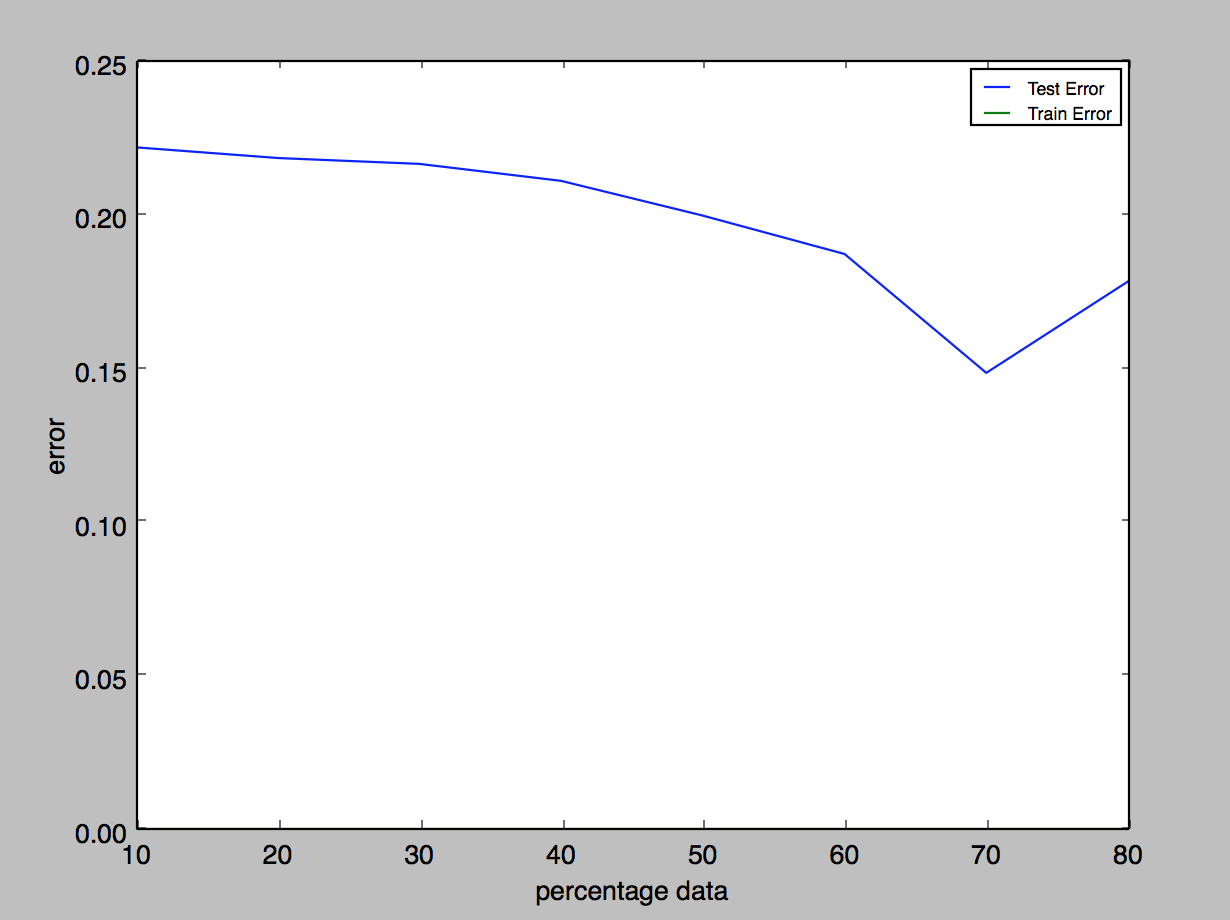
\includegraphics[scale=0.7]{learningcurve}

Note that the training set error is always at 0.0, presumably because it is linearly separable and thus can be 
perfectly fit. The large separation between the train and test sets tells us that we are in high variance, and 
thus want to decrease our hypothesis space and/or increase regularization.

So, we did a sweep of parameters to see how various different changes would perform. We looked at 
both RBF and linear kernels (linear would be better for high variance, but, experimenting with decreasing the number of features, it seemed possible we might get to a place where RBF performed well again), and $c$
and $\gamma$ values as before. However, we also considered three further changes to our features. The 
first was limiting the words used to the top $k$ most common, where $k$ was varied between 100 and the whole
set of vocab (about 1800 words). The second was removing English stop words, very common words that don't add much meaning. The third was using a TF-IDF transformer, also to try to decrease the importance of frequent but meaningless words. We used ScikitLearn's CountVectorizer and TfidfVectorizer to create our document term matrices using these parameters. 

We ran tests using \texttt{performance\_CI} written in a previous part on features and classifiers created with each combination of these parameters, and picked based on the highest accuracy score. We consistently found that limiting the number of features had a positive effect, but stop words and Tfidf had either negative or no effects one. We guess would be that this is because twitter users, with the character constraint, may use less meaningless common words than traditional language. In the end, our best model was as follows:
\\$C=10.0$
\\$\gamma = 0.001$
\\Number of Features = 500
\\Kernel = RBF
\\ Tfidf used = False

\begin{tabular}{| c | c | c | c |}
\hline
Metric & Score & Lower & Upper \\
\hline
Accuracy & $0.8571$ & $0.7714$ & $0.9286$ \\
F1-score & $0.9057$ & $0.8431$ & $0.9630$ \\
auroc & $0.8287$ & $0.6678$ & $0.9501$ \\
precision & $0.8727$ & $0.7777$ & $0.9536$ \\
sensitivity & $0.9412$ & $0.875$ & $1.0$ \\
specificity & $0.6316$ & $0.4167$ & $0.8500$ \\
\hline
\end{tabular}

When we compare this to our earlier results without feature selection, we see that it is better for all metrics
except for specificity, where is slightly lower than our best. This is likely because specificity is incredibly high. However, it still performs reasonably well, and the scores are high enough overall that we are happy. 

\end{enumerate}



\end{document}